 \documentclass[%
 aps,
 prl,%
 amsmath,amssymb,
%preprint,%
 reprint,%
%author-year,%
%author-numerical,%
]{revtex4-1}

\usepackage{graphicx}% Include figure files
\usepackage{dcolumn}% Align table columns on decimal point
\usepackage{bm}% bold math
%My packages start
%\usepackage{subfig}
\usepackage{multirow}					
\usepackage{array}
%\usepackage{booktabs}
\usepackage{footnote} 
\newcommand{\angstrom}{\text{\normalfont\AA}}
\usepackage{booktabs}
\usepackage{float}
\usepackage{mathtools}
\usepackage{color}
\newcommand{\comment}[1]{\noindent \textcolor{blue}{#1}}
%My packages end
%\usepackage[mathlines]{lineno}% Enable numbering of text and display math
%\linenumbers\relax % Commence numbering lines

\begin{document}

\title[]{Accelerating atomic structure search with cluster regularization}% Force line breaks with \\

\author{K.\ H.\ S{\o}rensen}
\author{M.\ S.\ J{\o}rgensen ??}
\author{B.\ Hammer}
\email{hammer@phys.au.dk}
\affiliation{ 
Department of Physics and Astronomy, and Interdisciplinary Nanoscience Center (iNANO), Aarhus University, Denmark.
}
% \homepage{phys.au.dk}
 
\date{\today}% It is always \today, today,
             %  but any date may be explicitly specified

\begin{abstract}
Knowing the atomic minimum energy structure for a material is very important for predicting 
its properties, but finding the atomic minimum structure is a difficult problem where the search can get stuck in many local minimums. 
While working with clustering on atomic feature vectors it was discovered that the sum of distances to cluster centers 
was correlated with the energy of the structures. Then the discovery was exploited in a regularization method which can help release the search from local minima.
The method was implemented as a mutation operator for the genetic search algorithm in the Atomic Simulation Environment (ASE) and then used to speed up the global minimum search for TiO$_{2}$ ridge reconstruction. 
\end{abstract}

\pacs{Valid PACS appear here}% PACS, the Physics and Astronomy
                             % Classification Scheme.
\keywords{}%Use showkeys class option if keyword
                              %display desired
\maketitle

\section{\label{sec:introduction}Introduction}
Evolutionary algorithms is frequently use in search for stable atomic structures and potential energy surfaces.

\section{The method}
What we are contributing in this article is a method we call cluster regularization. 
It is a way to impose symmetry into the search with out specifying the symmetry explicit, 
as pointed out in \cite{Pikard2011} low energy structures tend to have a very high degree of symmetry.

The method first constructing a feature vector for each atom, then cluster this feature vectors, and at last change the atomic positions such that the distance between the feature vectors and the cluster centers are minimized.   


\subsection{Atomic features}
 
The atomic features vectors used in this study is inspired from Botu and Ramprasad \cite{Boto2015} and also used by Xin Chen \cite{Chen2017}.

The length of our feature vector is the number of atomic types plus one. For our system with 2 atomic types the atomic feature vector have length 3.

The first 2 components for each atom $i$, is calculated by finding the list of neighbors $nl(i)$ within a cutoff radius $c$. For each of the 2 atomic types T we calculate. 

\begin{equation}
f_T(i) = \sum_{\mathclap{j \in nl(i,c);T=T(j)}} e^{-r_{ij}/1\text{\AA}}f_c(r_{ij})  \label{eq1}
\end{equation}

Here T(j) is the atomic number of the j'th atom. $r_{ij}$ is the distance from the i'th to the j'th atom in {\AA}ngstr\"{o}m. The last component of the atomic feature vector is $T(i)$ the atomic number for atom i. 
The function $f_c$ make sure that an atoms contribution vanish at the cut-off radius, this gives the gradient higher stability.

\begin{equation}
f_c(r)={{\cos(\pi*r/c)+1}\over 2}
\end{equation}



In figure \ref{fig1} the feature vector is displayed for 1019 structures of Ti$_{13}$O$_{26}$ with the first component $f_8(i)$ along the x-axis, the second $f_{22}(i)$ along the y-axis and the color is given by the third component $T(i)$. 


\begin{figure}[h]
    \centering
    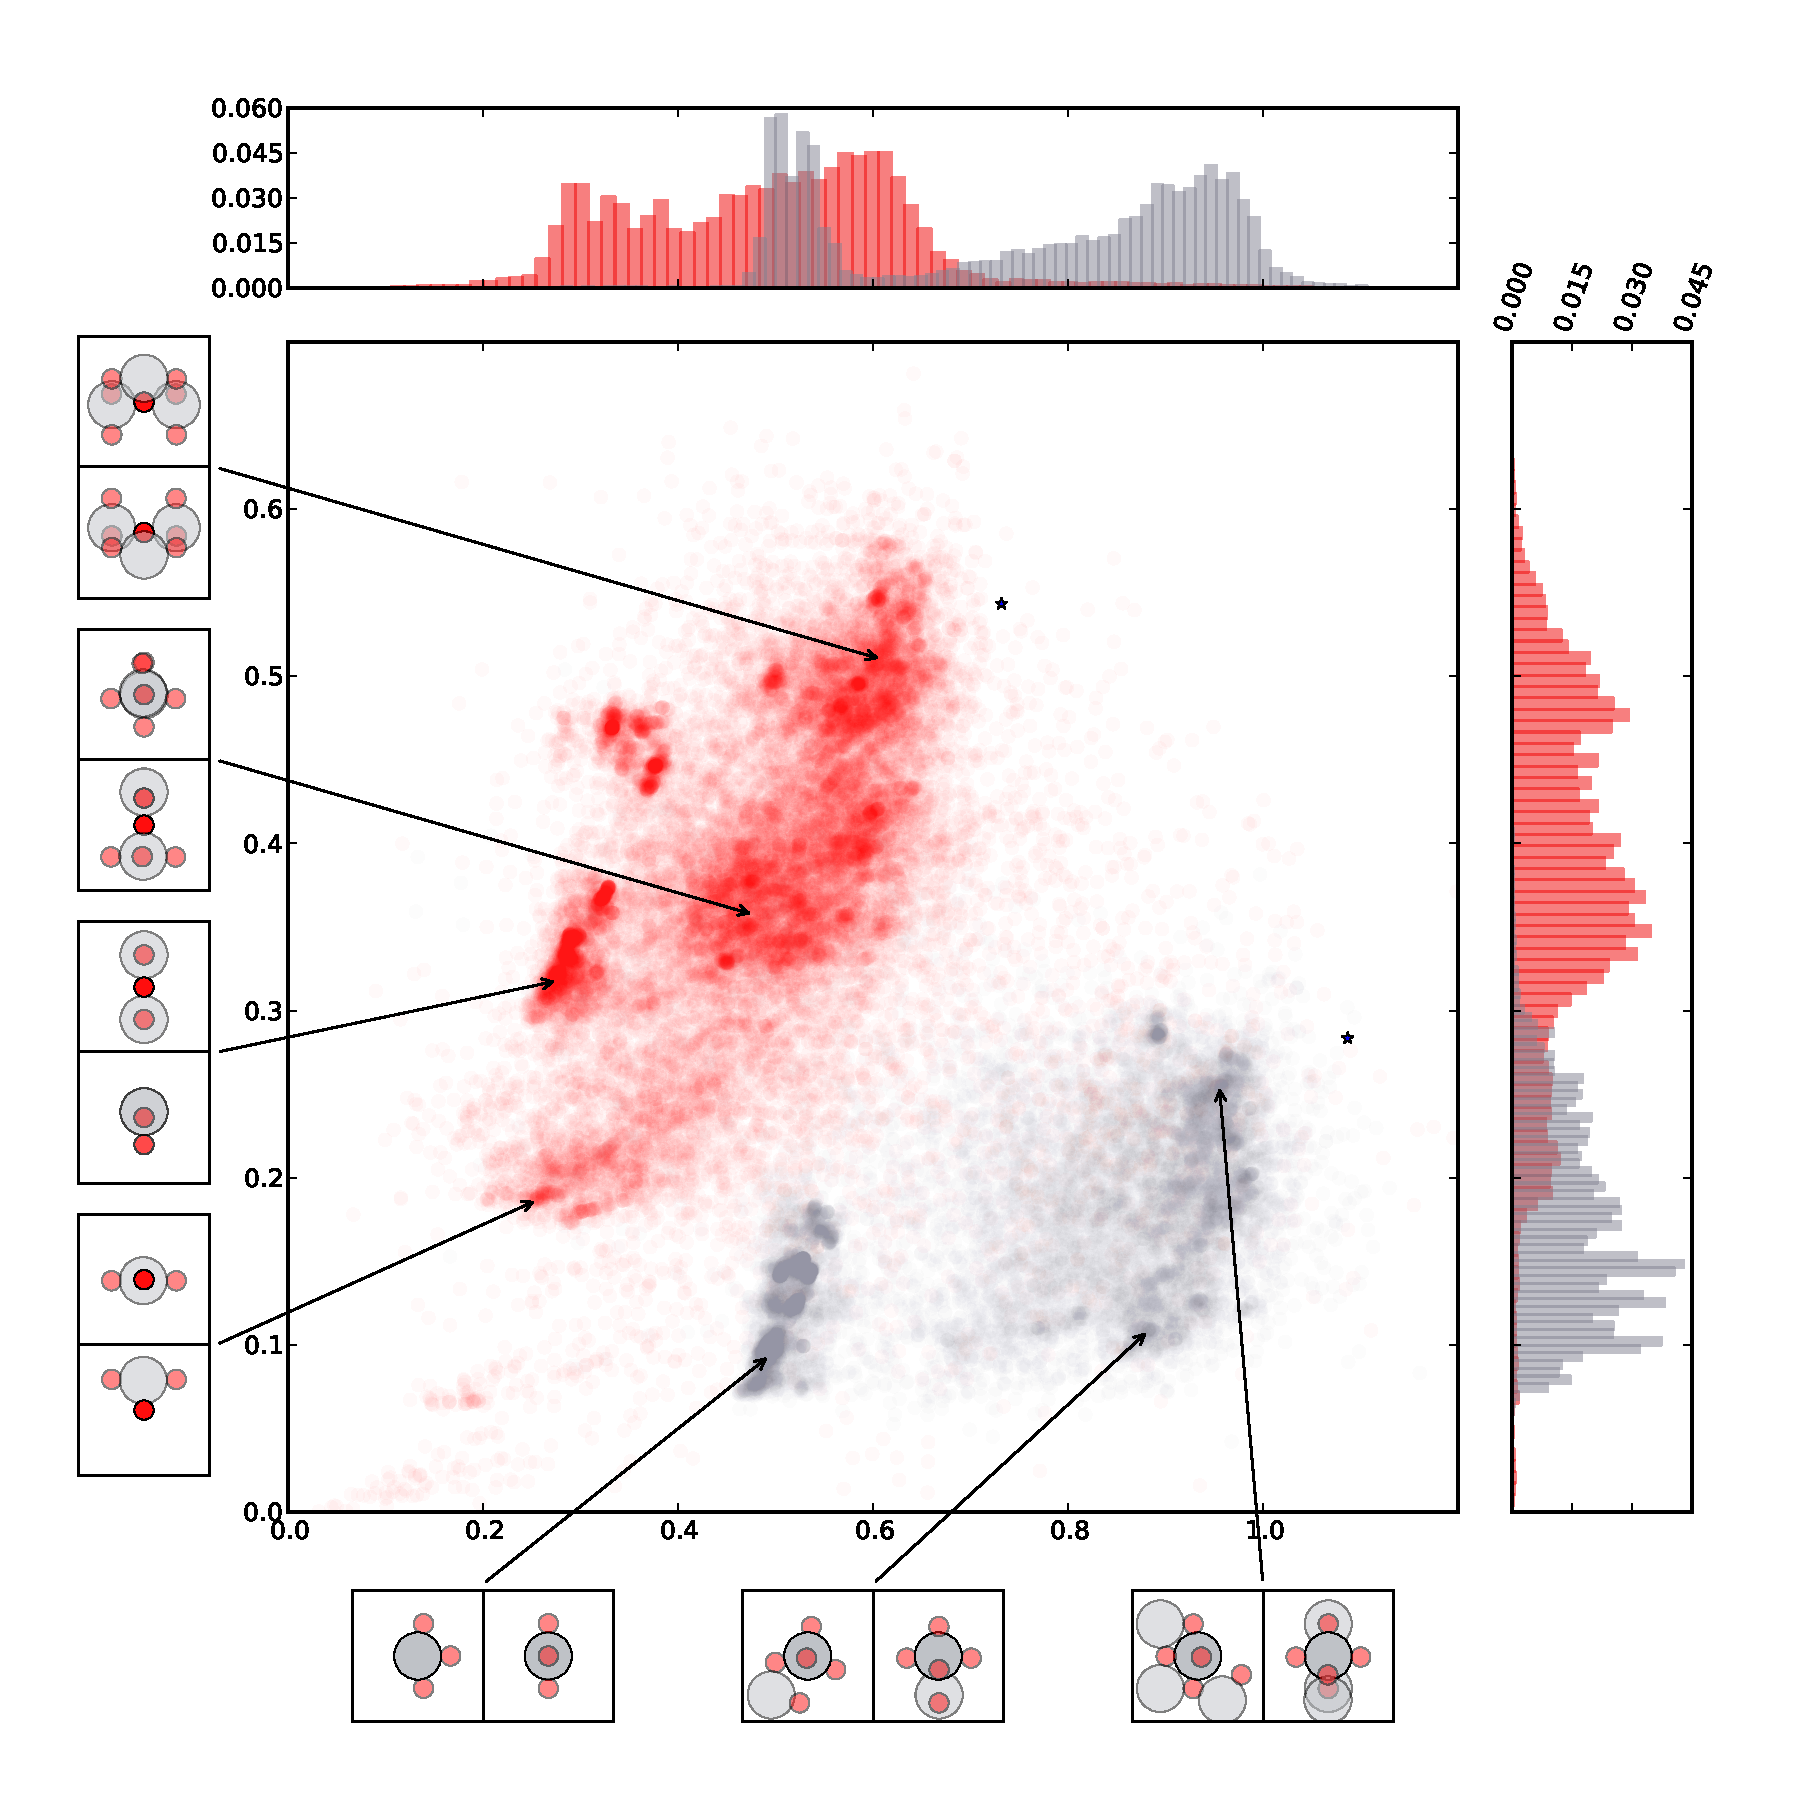
\includegraphics[width=1.0\columnwidth]{fig1-scatterplot.pdf}
    \caption{Visualization of atoms from 1019 Ti$_{13}$O$_{26}$ structures in feature space}
    \label{fig1}
\end{figure}


\subsection{Clustering}
The clustering method used is this study is k-means with 2
modifications. The first is a modification to avoid generating empty
clusters \cite{Malay2009} and the second modification is using
k-means++ cluster initialization. While working with clustering on the
atomic feature vectors, the total cluster distance vs. energy correlation
illustrated on figure \ref{fig_corr} was discovered. 

\begin{figure}[h]
    \centering
    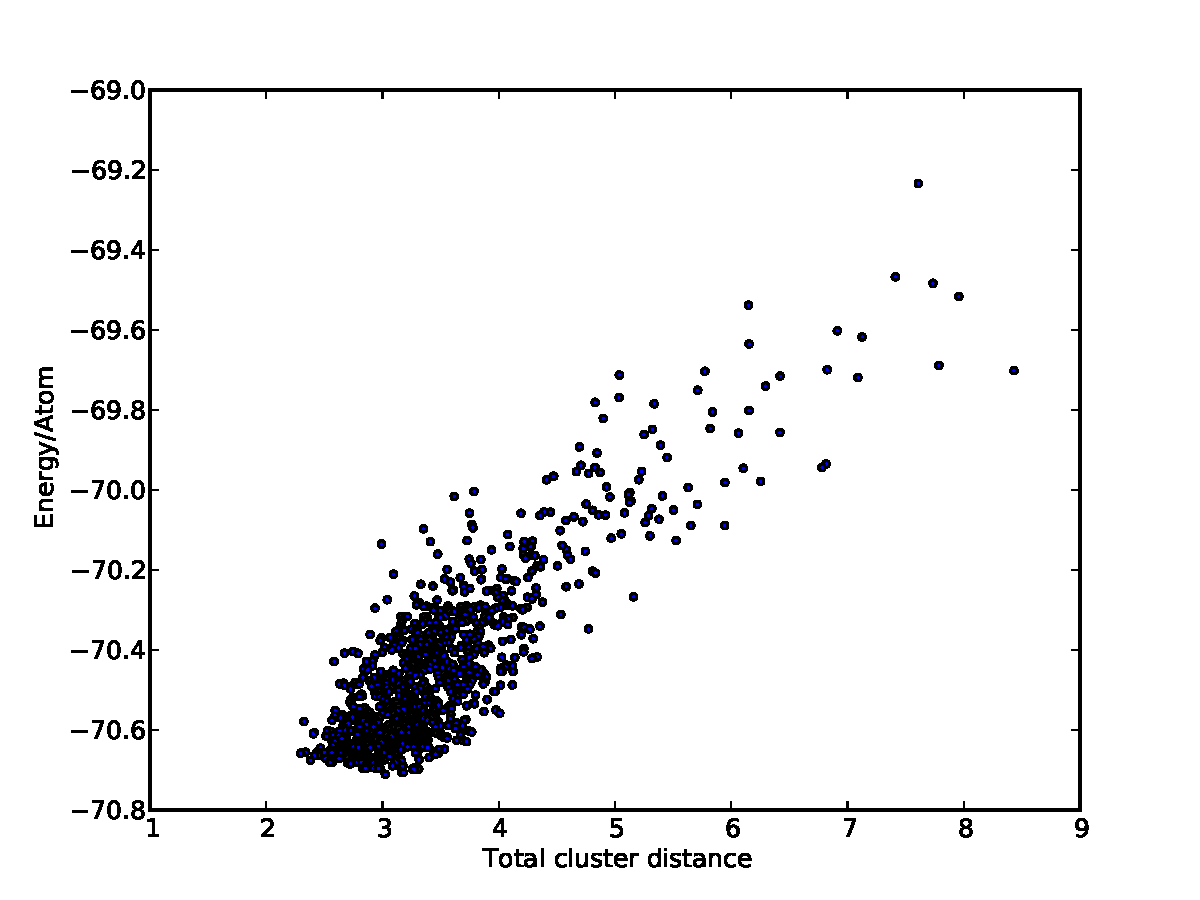
\includegraphics[width=1.0\columnwidth]{decoorL2_5_fgen_Ti13O26Ridge_9_11_9_1510066208.pdf}
    \caption{Cluster distance vs. energy correlation}
    \label{fig_corr}
\end{figure}

It was immediately recognized that it could be applied to speed up the search for minimum energy structures.
It is our suspicion that the better the correlation the higher the speedup, 
but we haven't done a formal study of this. We have observed that regular structures like bunk and surface have better correlation than molecules. Another factor influencing the correlation is the choice of feature vector, 
unlike other machine learning methods this type of clustering don't ignore noisy features, so the features should be chosen with care.  
 
Given an atomic structure $S$ (a list of atoms) the total cluster distance is given by:
\begin{equation}
\text{TCD}(S) = \sum_{i \in S} d(\vec f(i), \vec c(\vec f(i))) \label{eq3}
\end{equation}
For each atom $i$ in $S$ we calculate the feature vector $\vec f(i)$ then 
assign it to a cluster center $\vec c(\vec f(i))$.   
The sum over the distance between $\vec f(i)$ and $\vec c(\vec f(i))$ for all atoms $i$ in a structure $S$ 
gives the total cluster distance $TCD(S)$.
In the case of figure \ref{fig_corr} the cluster centers is found by clustering over all atomic feature vectors 
for the 1019 structures in the data set. 

\subsection{Cluster regularization}

Because the all but the last components of our feature vector is analytical functions of the atomic coordinates, one can derive the analytical gradient. Now we can minimize the cluster distance by following the negative gradient to a local minima. Then we switch and minimize the energy with DFTB+ and then minimize cluster distance again. Figure \ref{fig_min} shows the process. The idea is that alternate the two minimizations they will help each other out of there local minima and further down in energy and cluster distance.
   
\begin{figure}[h]
    \centering
    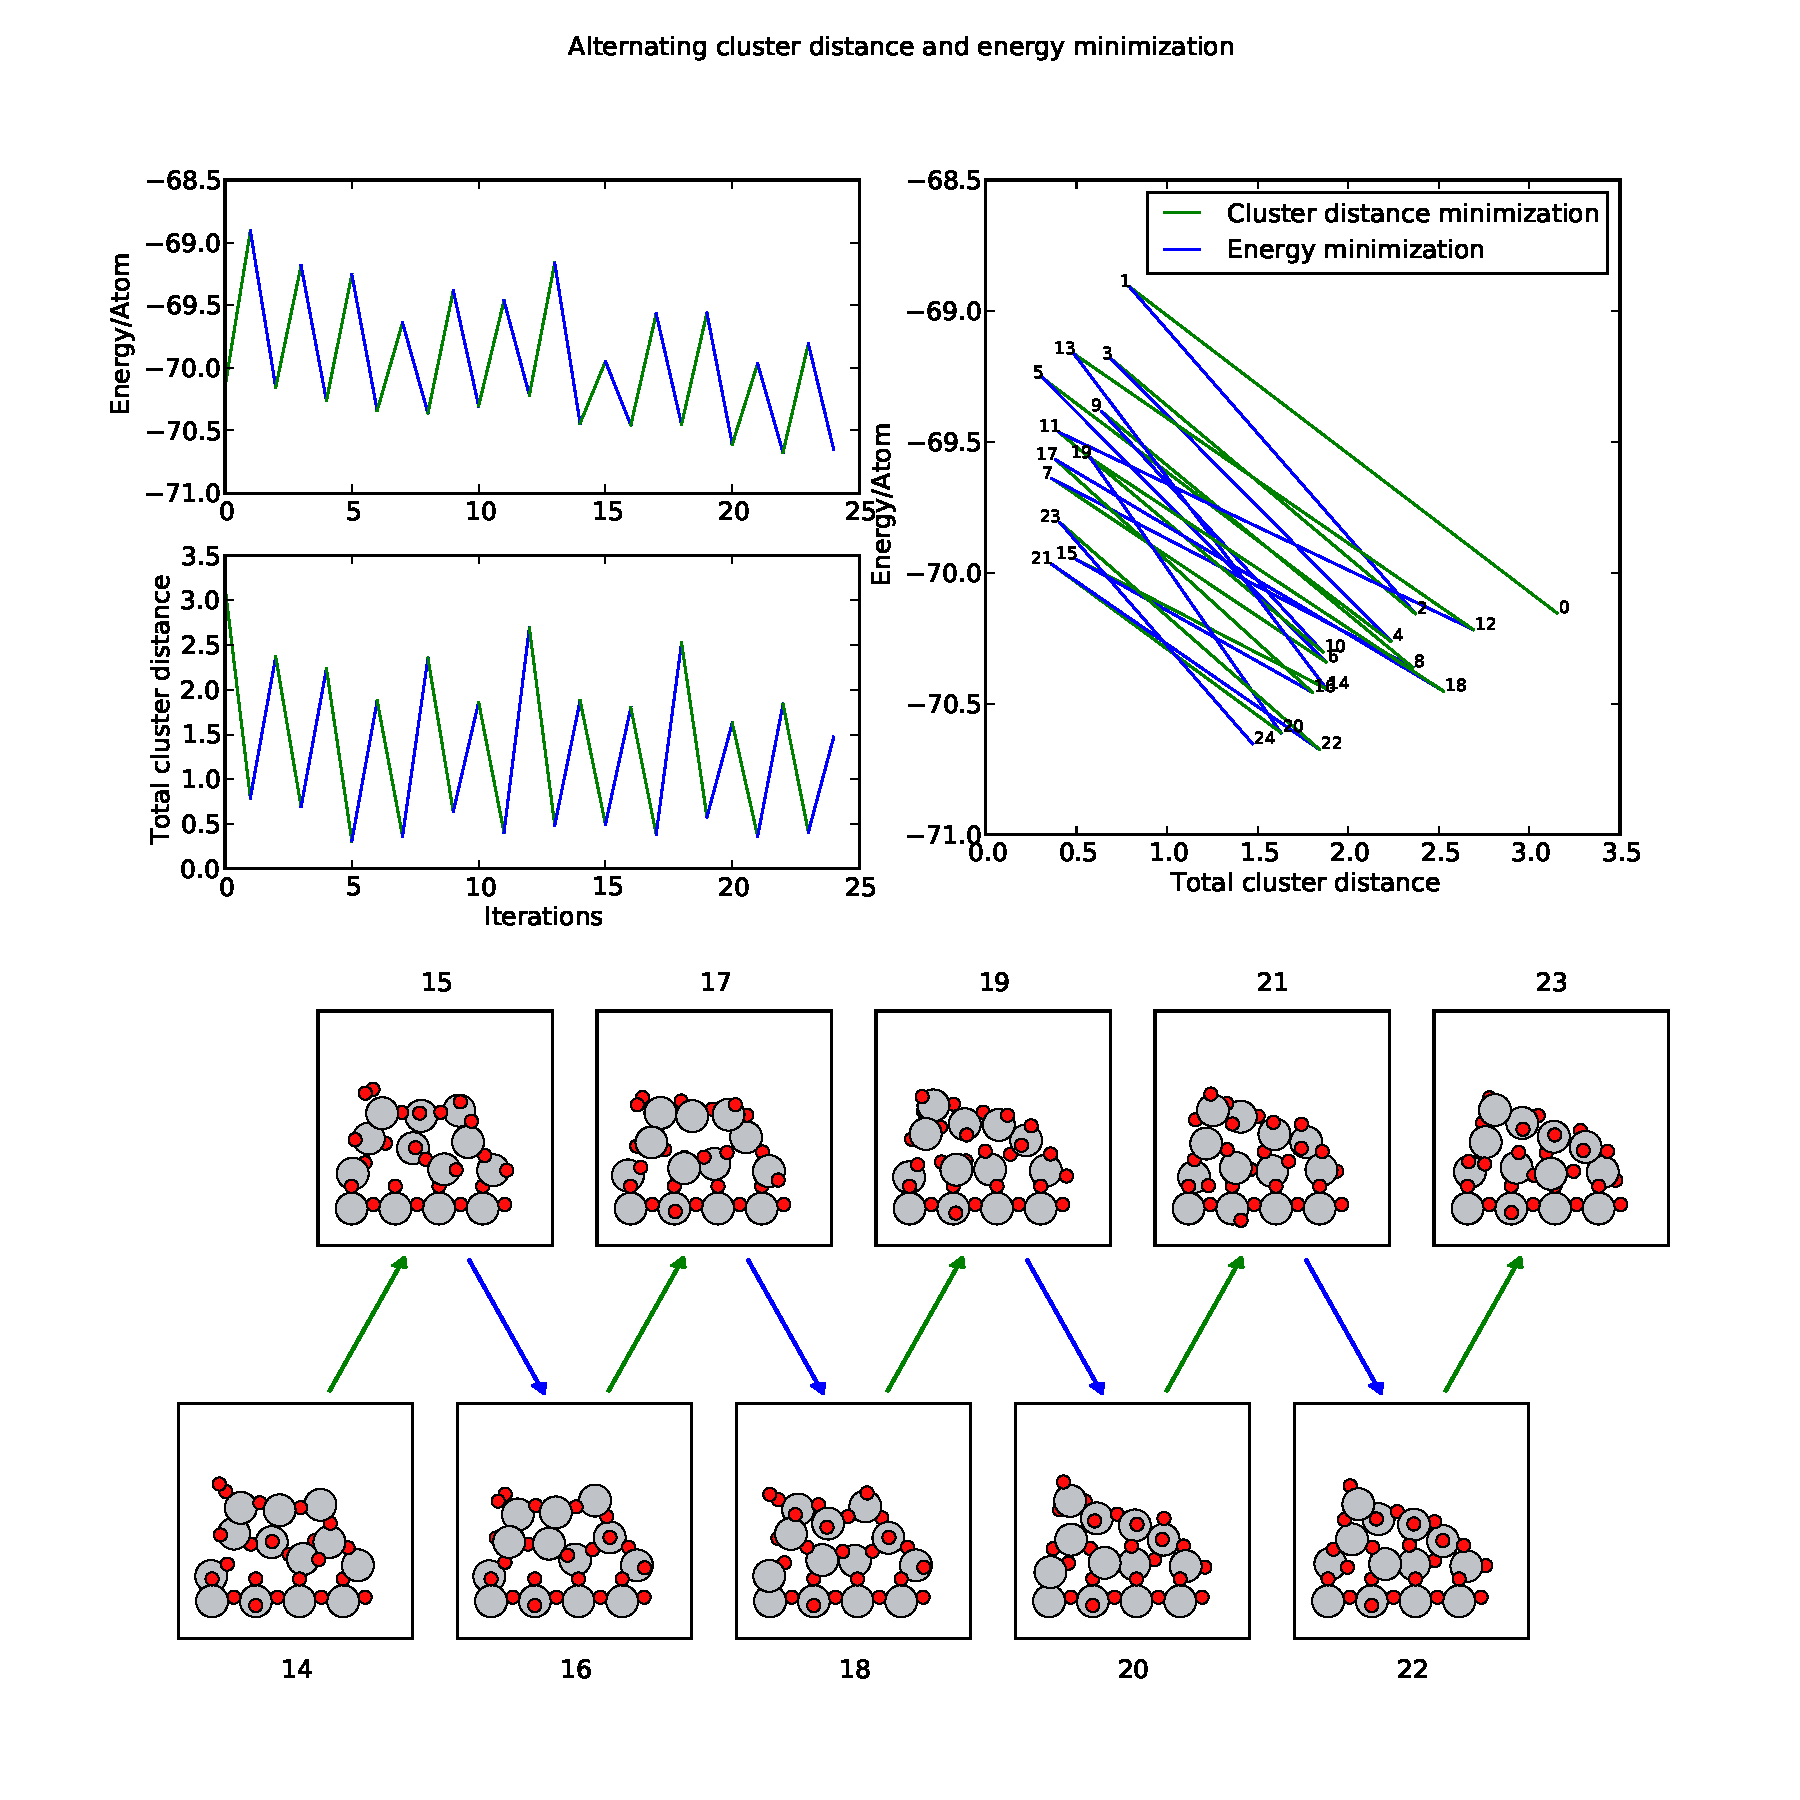
\includegraphics[width=1.0\columnwidth]{acdminplot_74_98_ridgemin2_5_9_500_Ti13O26Ridge.pdf}
    \caption{Green lines and arrows shows a cluster distance (cd) minimization and the blue DFTB+ relaxations. Here the first/bottom layer is the template. While it is hard to see progress in individual minimization step there is small details to notice on the plot. Notice that in the cd. step from 16 to 17 the hole in the second layer is filled and that in the cd. step from 18 to 19 the 2 oxygen atoms in top left corner is split up.}
    \label{fig_min}
\end{figure}


\section{Testing}

\subsection{Test setup}
To test the technique we implemented cluster regularization as a mutation operator in ASE's genetic algorithm (ga)\cite{ase_ga} framework. 
The mutation operator takes a list of parents and the execute the following steps:
\begin{enumerate}
\item Calculate atomic features for all parents.
\item Cluster them and find cluster centers.
\item Copy the lowest energy parent to the child
\item minimize cluster distance of child.
\item return child.
\end{enumerate}
When the mutation returns the child then the ga will make a energy relaxation 
and we have a cycle as illustrated in figure \ref{fig_min}.

To establish a benchmark the ga with bayesian hyper-parameter optimization (bho) search was run on the 3 layer system.
Run with cut\&splice, permutation and rattle mutations the search found the optimal ratios was 59\% cut\&splice, 0\% permutation, 41\% rattle. 

Next we did a bho search for the best parameters for cluster regularization, we found that 5 clusters, 3 parents and cutoff radius c=11.9 gave the best results.

Last we did a bho search for the best combination of cluster regularization, cut\&splice and rattle, we found that 70\% cluster regularization, 28\% cut\&splice and 2\% rattle did well.

We tested these 3 configuration on a 2 layer, 3 layer and a 4 layers system. 

\section{Test result}

On figure \ref{2lfig} we see that pure cluster reg. (orange curve) start finding minimum structure much faster than the benchmark (yellow curve) , but it levels out around 60-70\%. The problem is that cluster regularization and energy minimization have local minima close to each other and running the algorithm make them switch between this minima. When cluster regularization is mix with other mutations (red cure) the problem disappear. 

\begin{figure}[h]
    \centering
    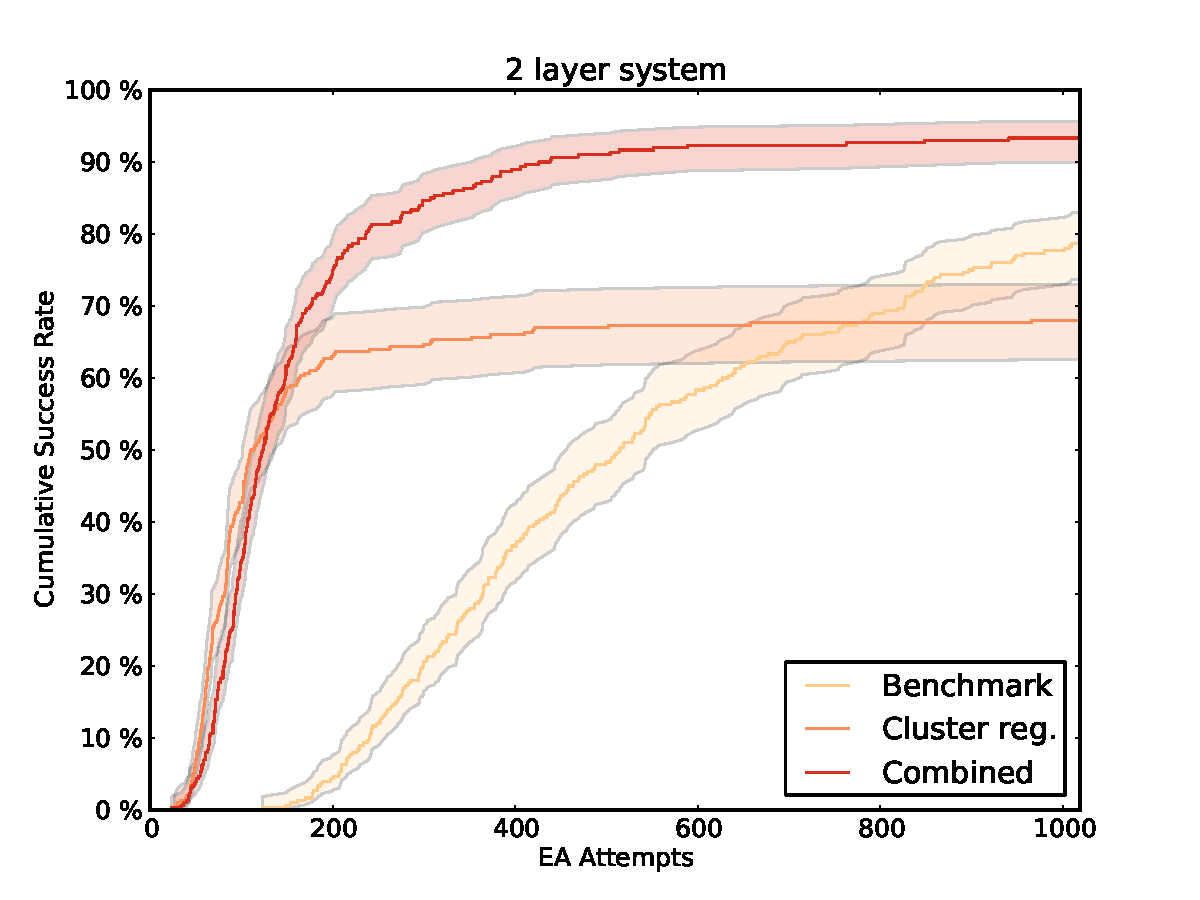
\includegraphics[width=1.0\columnwidth]{2lsuccess.pdf}
    \caption{Cumulative success for 2 layer system}
    \label{2lfig}
\end{figure}

With the 3 layers system on figure \ref{3lfig} the problem isn't as prominent which might be because there is more free variables in this problems. Else we observe the same as the 2 layer system combined and pure cluster reg. does better than benchmark. Pure cluster reg. does better in the start but is overtaken by the combined method later on. 
 

\begin{figure}[h]
    \centering
    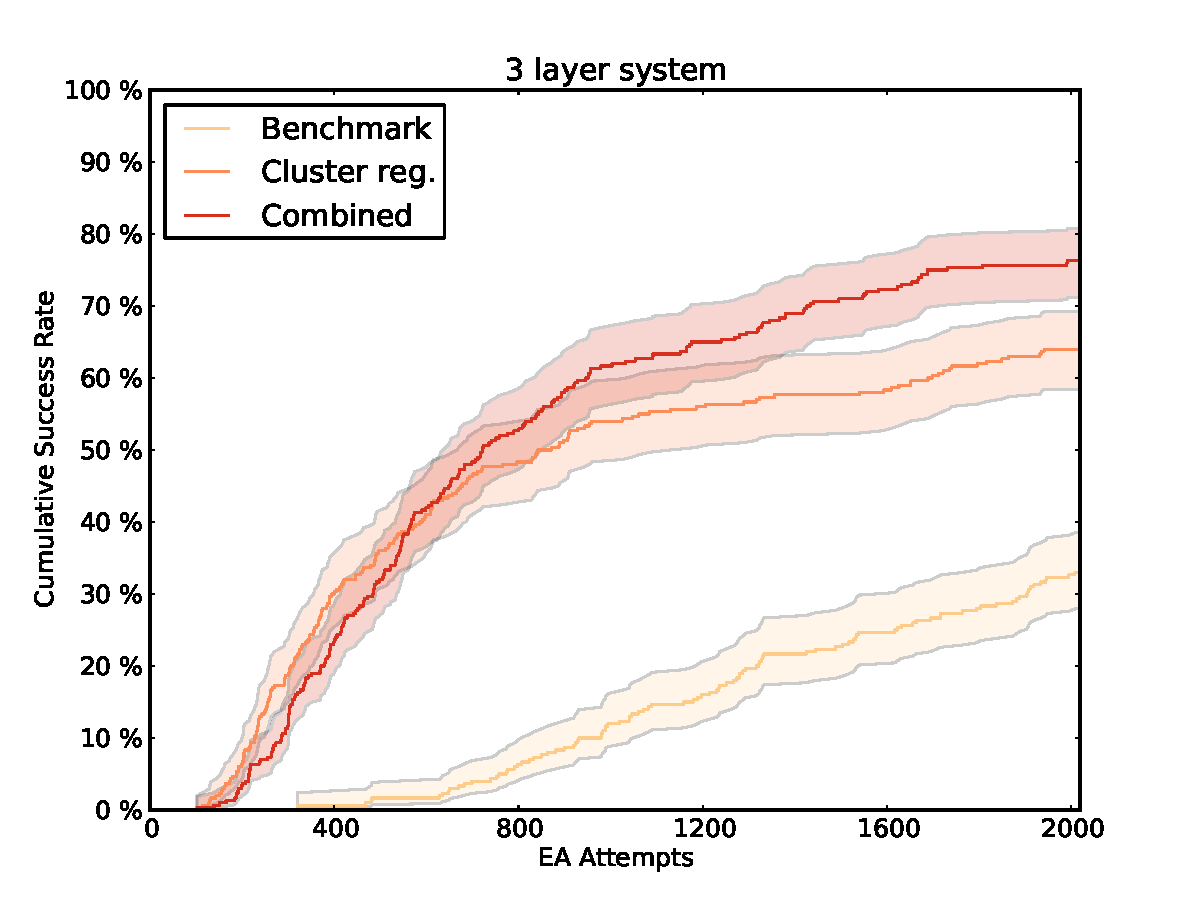
\includegraphics[width=1.0\columnwidth]{3lsuccess.pdf}
    \caption{Cumulative success for 3 layer system}
    \label{3lfig}
\end{figure}

In the 4 layer system the tendency continues but the success rate is much lower and we made double as many runs to shrink the confidence intervals. 

\begin{figure}[h]
    \centering
    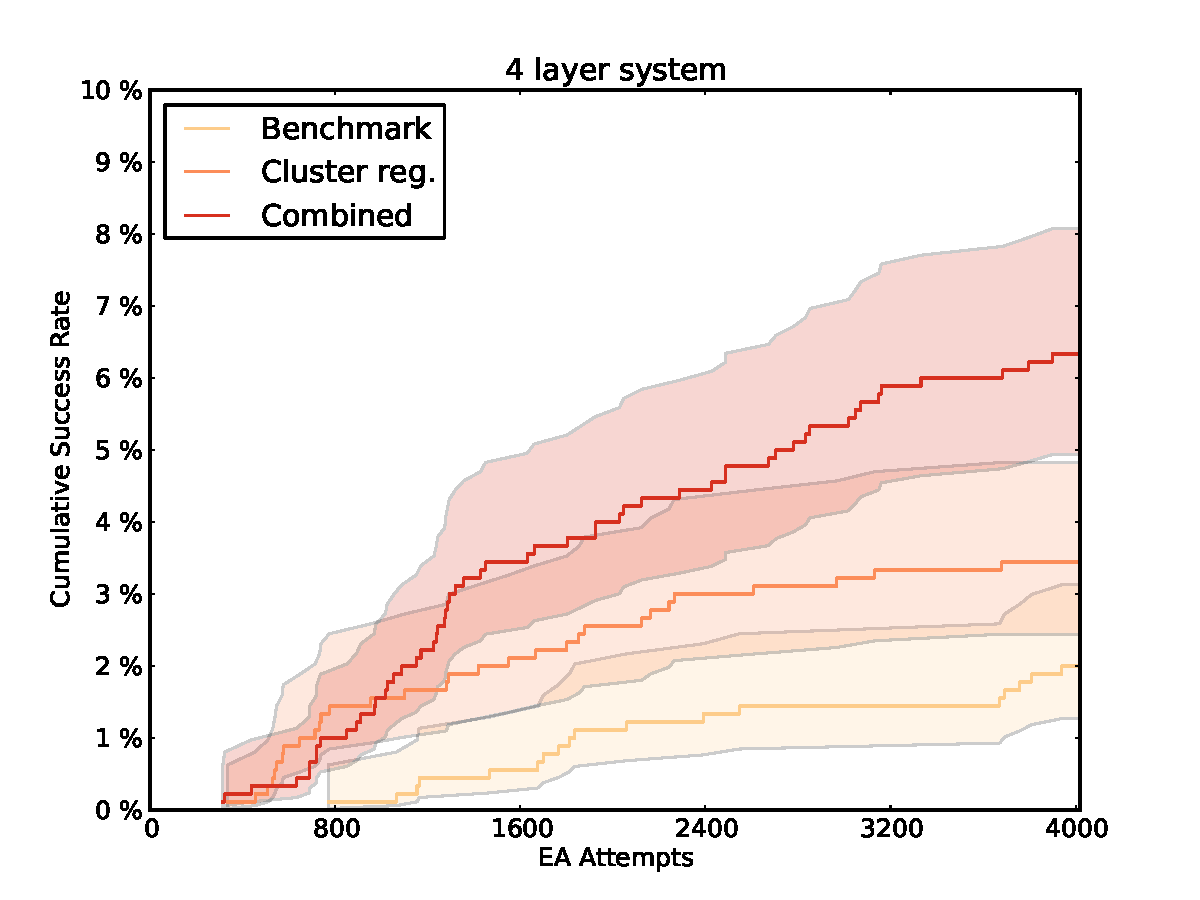
\includegraphics[width=1.0\columnwidth]{4lsuccess.pdf}
    \caption{Cumulative success for 4 layer system}
    \label{4lfig}
\end{figure}


We acknowledge support from the Danish Research Council (grant no. 0602-02566B) and from VILLUM FONDEN (Investigator grant, project no. 16562).

\begin{thebibliography}{12}  
  \bibitem{Starke1998} U. Starke \textit{et al}., Phys. Rev. Lett. \textbf{80}, 758 (1998).    
  \bibitem{Botu2015} {Adaptive Machine Learning Framework to Accelerate Ab Initio Molecular Dynamics.} V. Botu and R. Ramprasad, Int. J. Quantum Chem. 2015, 115 ,1075-18083. DOI:10.1002/qua.24836    
 \bibitem{Malay2009} {A Modified k-means Algorithm to Avoid Empty Clusters} Malay K. Pakhira, International Journal of Recent Trends in Engineering, Vol 1, No 1, May 2009
 \end{thebibliography}


\end{document}
